%& -shell-escape

%%% Copyright (c) 2011, Илья w-495 Никитин
%%%
%%% Разрешается повторное распространение и использование
%%% как в виде исходного кода, так и в двоичной форме,
%%% если таковая будет получена, с изменениями или без, 
%%% при соблюдении следующих условий:
%%%
%%%     * При повторном распространении исходного кода 
%%%       должно оставаться указанное выше уведомление 
%%%       об авторском праве, этот список условий
%%%       и последующий отказ от гарантий.
%%%     * Ни имя w-495, ни имена друзей или консультантов
%%%       не могут быть использованы в качестве поддержки
%%%       или продвижения продуктов, основанных на этом коде 
%%%       без предварительного письменного разрешения. 
%%%
%%% Этот код предоставлен владельцом авторских прав 
%%% и/или другими сторонами <<как она есть>> 
%%% без какого-либо вида гарантий, выраженных явно 
%%% или подразумеваемых, включая, но не ограничиваясь ими, 
%%% (подразумеваемые) гарантии коммерческой ценности и пригодности 
%%% для конкретной цели. Ни в коем случае, если не требуется 
%%% соответствующим законом, или не установлено в устной форме, 
%%% ни один владелец авторских прав и ни одно другое лицо,
%%% которое может изменять и/или повторно распространять программу,
%%% как было сказано выше, не несёт ответственности,
%%% включая любые общие, случайные, специальные 
%%% или последовавшие убытки, вследствие использования 
%%% или невозможности использования программы 
%%% (включая, но не ограничиваясь потерей данных, 
%%% или данными, ставшими неправильными, или потерями
%%% принесенными из-за вас или третьих лиц, 
%%% или отказом программы работать совместно 
%%% с другими программами), даже если такой владелец или другое
%%% лицо были извещены о возможности таких убытков.
%%% 

%%% Документ нужно собирать только в XeLaTeX:
%%% 	$>xelatex имя-файла.tex
%%% Для этого должны быть установлены пакеты XeLaTeX и XeTeX
%%% 	в TeXLive или MikTeX или иной, 
%%% если она поддерживает последние обновдения CTAN.


\documentclass[unicode, 12pt, a4paper,oneside,fleqn]{article}
	%% Варианты []:
		% fleqn --- сдвигает формулы влево

	%% Варианты {}:
		% book
		% report
		% article
		% letter
		% minimal (???)

\usepackage{styles/init} 
	% подключаем набор стилей 
	% там были определены базовые настройки шрифтов
	% и пакетов роботы с графикой и листингами
	
	% При не обходимости шрифты следует переопределить
	% потому что, если в Вашей системе 
	% не окажется нужных шрифтов, pdf не соберется
	
	% текущее положение включаемых файлов --- ./src

	\hypersetup{ 
		unicode=false,
		% %	pdffitwindow=false,
		% % pdfstartview={FitH}, % как отображать страницу {FitH}, {FitW}
		pdftitle={Это шаблонный документ XeTeX v0.35}, 
		pdfauthor={Илья w-495 Никитин},
		pdfcreator={XeTeX + TexMaker + w-495}, 
		pdfsubject={Тема}, 
		pdfproducer={w-495}, 
		pdfkeywords={Шаблон}
	}

\begin{document}

%%%%%%%%%%%%%%%%%%%%%%%%%%%%%%%%%%%%%%%%%%%%%%%%%%%%%%%%%%%%%%%%%%%%%%%%%%%%%%%%
%%%
%%% бесполезное содержимое
%%%

	\begin{titlepage}
\begin{center} %% ПО ЦЕНТРУ

\bfseries
%%%%%%%%%%%%%%%%%%%%%%%%%%%%%%%%%%%%%%%%%%%%%%%%%%%%%%%%%%%%%%%%%%%%%%%%%%%%%%%%
%%%
%%% ВУЗ
%%%

	{\Large Московский авиационный институт \\
	(государственный \TeX нический университет)
	
	} %% или что-то в этом духе

\vspace{48pt}

%%%%%%%%%%%%%%%%%%%%%%%%%%%%%%%%%%%%%%%%%%%%%%%%%%%%%%%%%%%%%%%%%%%%%%%%%%%%%%%%
%%%
%%% Факультет
%%%

	{\large Факультет прикладной математики
	
	}

	%{\large Факультет иностранных языков
	%
	%}

\vspace{36pt}
%%%%%%%%%%%%%%%%%%%%%%%%%%%%%%%%%%%%%%%%%%%%%%%%%%%%%%%%%%%%%%%%%%%%%%%%%%%%%%%%
%%%
%%% Кафедра
%%%


	{\large  {\comic Кафедра вычислительной математики и~программирования}
	
	} %% или что-то в этом духе

\vspace{48pt}
%%%%%%%%%%%%%%%%%%%%%%%%%%%%%%%%%%%%%%%%%%%%%%%%%%%%%%%%%%%%%%%%%%%%%%%%%%%%%%%%
%%%
%%% Класс работы
%%%

	{\large	\DoloresCyr Шаблон по курсу <<Какой-то предмет>> 
	
	}
	% Лекции по курсу \enquote{Какой-то предмет} 
	% Лабораторная работа по курсу \enquote{Какой-то предмет} 
	% Курсовая работа по курсу \enquote{Какой-то предмет} 
	% Курсовой проект по курсу \enquote{Какой-то предмет} 

\vspace{12pt}
%%%%%%%%%%%%%%%%%%%%%%%%%%%%%%%%%%%%%%%%%%%%%%%%%%%%%%%%%%%%%%%%%%%%%%%%%%%%%%%%
%%%
%%% Название работы
%%%

	%{\Large <<Какое-то название>> 
	%}

\end{center} %% УЖЕ НЕ ПО ЦЕНТРУ

\vspace{60pt}
%%%%%%%%%%%%%%%%%%%%%%%%%%%%%%%%%%%%%%%%%%%%%%%%%%%%%%%%%%%%%%%%%%%%%%%%%%%%%%%%
%%%
%%% Автор(ы)
%%%

	\begin{flushright}
		\begin{tabular}{rl}
			Студент: & И.\,К. Никитин \\
			Преподаватель: & Э.\,И. Иванов \\
		\end{tabular}
	\end{flushright}

\vfill
%%%%%%%%%%%%%%%%%%%%%%%%%%%%%%%%%%%%%%%%%%%%%%%%%%%%%%%%%%%%%%%%%%%%%%%%%%%%%%%%
%%%
%%% Дата
%%%

	\begin{center} %% ПО ЦЕНТРУ
		\bfseries
		Москва, 2010
	\end{center}
	
\end{titlepage} 

 	% титульный лист
	\tableofcontents 		% оглавление
	\pagebreak

	%%%%%%%%%%%%%%%%%%%%%%%%%%%%%%%%%%%%%%%%%%%%%%%%%%%%%%%%%%%%%%%%%%%%%%%%%%%%%%%%
	%%%
	%%% дополнительное (свое) задание верхнего колонтитула
	%%% 
	%%%
	%	\makeatletter
	%	\renewcommand{\@oddhead}{ \textcolor{blue}{Лекция (задача) \arabic{lections}} \hfil \par
	%	\hfil  \leftmark \hfil \rightmark }
	%	\makeatother

	
%%%%%%%%%%%%%%%%%%%%%%%%%%%%%%%%%%%%%%%%%%%%%%%%%%%%%%%%%%%%%%%%%%%%%%%%%%%%%%%%
%%%
%%% полезное содержимое
%%%

	% пример %%%%%%%%%%%%%%%%%%%%%%%%%%%%%%%%%%%%%%%%%%%%%%%%%%%%%%%%%%%%%%%%%%%
	% это просто пример, который, якобы может показать основные особенности, 
	% фичи и недостатки, 
	
	\Csection{Введение}

Эпоха думающих машин и проблемы человечества.
Человек уже давно начал задумываться об интеллекте и разуме. Что-же такое интеллект? Как его можно описать? Где он расположен? Из чего состоит собственное ``Я'' каждого человека? Над этими вопросами работали и работают большое количество философов, учёных и инженеров. И судя по всему до окончательного ответа ещё очень далеко.

Мы живём в век продолжающегося бурного развития компьютеров и компьютерной техники. За последние пятьдесят лет произошёл стремительный взлёт информационно-вычислительной техники. В 1905 году Джон Флеминг запатентовал ``прибор для преобразования переменного тока в постоянный'' --- первую электронную лампу. Вакуумные электронные лампы стали элементной базой для компьютеров первого поколения. В 1960-м году после работ американцев Канга и Аталлы, на основе кристалла кремния был впервые изготовлен полевой транзистор. Вычислительная техника стала стремительно дешеветь, уменьшаться в размерах, стало сокращаться энергопотребление и вместе с тем начала расти производительность вычислений. Позже возникли интегральные схемы, что в свою очередь ещё более расширило возможности вычислительной техники. Появились языки программирования, стало возможным писать большие и сложные программы которые уже стали представлять не только академический, но уже и практический интересы. Люди стали задумываться: нельзя ли написать такую программу, собрать такую схему чтобы получить уже электронный интеллект?

Эта работа представляет попытку произвести краткий обзор того, что человечеству удалось добиться в создании думающих машин и тех результатов, которых удалось достичь.

\pagebreak

	%\supersection{Техника и философия}
        \section{Техника и философия}
С давних времён человека сопровождает техника, но не сразу человеческая цивилизация стала технической. В ХХ веке в развитии техники произошёл качественный скачок, из-за этого техника стала предметом изучения философии. Немецкий философ Эрнст Капп и русский инженер Пётр Климентьевич Энгельмейер были первыми, кто начал рассуждать о проблемах техники и общества. С тех же пор сама техника, её развитие, место и роль в цивилизации стали предметами изучения. Не только философы, но и сами инженеры, начали уделять осмыслению техники все большее внимание. Часто такое осмысление сводится к исключительно оптимистической оценке достижений и перспектив ин\-фор\-ма\-цион\-но-тех\-ни\-чес\-ко\-го развития. 

В это же время в гуманитарной среде возросло критическое отношение к такому техническому прогрессу современного общества. В современной философии внимание привлекается, прежде всего, к отрицательным сторонам информационно-технического прогресса.  Технический прогресс породил в ХХ веке большое количество специальных технических дисциплин, которые исследуют различные аспекты техники. В то же самое время техника в целом не является предметом исследования технических дисциплин. Многие естественные науки вынуждены принимать во внимание технику, они делают её предметом специального исследования, конечно, со своей особой естественнонаучной, например, физической точки зрения. Кроме того, из-за проникновения техники практически во все сферы жизни человечества, многие общественные науки обращаются к специальному анализу технического развития. 

Философия техники исследует феномен техники в целом, её место в общественном развитии и уделяет особое внимание вопросам и проблемам, связанным с влиянием техники на человека.  Что же такое техника? Как можно интерпретировать это понятие. Для древних греков ``технэ'' (античное ``технэ'' – это не техника в нашем понимании, а все, что сделано руками: военная техника, игрушки, модели, изделия ремесленников и даже произведения художников) располагается ниже мудрости, и ключом для понимания ``технэ'' является знание общего. Сократ и Аристотель придерживались следующей точки зрения соотношения знаний философов и ремесленников: ``наставники более мудры не благодаря умению действовать, а потому что они обладают отвлеченным знанием и знают причины''.

В средние века техника сохраняет свое вторичное значение и считается результатом божественного творчества. В новое время желание человека господствовать над природой реализуется в технике, она представляется как продолжение науки, выступает как сила человеческого разума и результат его инженерных способностей. Карл Маркс приходит к выводу, что производственные силы, средства производства являются изначальным базисом общества. Средствами производства является техника. Особый интерес представляет понимание техники в ХХ веке, потому что именно в это время техника превратилась в силу, господствующую над человеком. Сейчас мы под техникой понимаем следующее:

\begin{itemize}
\item{совокупность технических устройств (от самых простейших орудий до сложнейших технических систем);}
\item{совокупность различных видов технической деятельности по созданию подобных устройств;}
\item{совокупность технических знаний.}
\end{itemize}

К сфере техники можно отнести не только использование, но и само производство научно-технических знаний, т.е. современная техника неразрывно связана с развитием науки. Техника включается в самостоятельную сферу жизнедеятельности, а именно в техносферу. ``Под техносферой понимается исторически обусловленная, сознательно формируемая, поддерживаемая и совершенствуемая система отношений между человеком и природой, человеком и техникой, человеком и человеком на основе определенного технического миропонимания''. Кроме техносферы философы рассматривают ноосферу. ``По мнению В.И. Вернадского, ноосфера — это гармоническое соединение природы и общества, это торжество разума и гуманизма, это слитая воедино наука, общественное развитие и государственная политика на благо человека, это — мир без оружия, войн и экологических проблем, это — мечта, цель, стоящая перед людьми доброй воли, это — вера в великую миссию науки и человечества, вооруженного наукой''.

Основоположники учения о ноосфере (В.И. Вернадский, П. Тейяр де Шарден) верили, что человеческий разум, превращаясь в планетарную геологическую силу, приведет к упорядочению природной и социальной действительности, к более совершенным формам бытия. Как результат планомерного, сознательного преобразования биосферы, ее перехода в качественно новое состояние возникнет ноосфера. Ноосфера связана с техносферой, так же как разум связан с техникой, потому что разум есть потенциальная техника, а техника есть актуальный разум. Движется ли современное человечество по пути, который приведет к ноосфере в понимании Владимира Ивановича Вернадского, или техносфера и ноосфера являются продуктами деятельности человечества и несут в себе гибель?

Русский философ Владимир Александрович Кутырев утверждает, что структурно, ноосфера и техносфера — синонимы, что можно, не разрушая категориальной сущности, продолжить этот ряд понятиями наукосферы, рациосферы, инфосферы, интеллектосферы. ``И все они, порождаясь природой, ``снимают'' ее, противостоят ей''. В.А. Кутырев видит в ноосфере утопию и рассматривает технику как средство уничтожения всего человеческого. Карл Ясперс при анализе техники сформулировал мысль о том, что человеку необходимо опасаться техники, он может ``потеряться в ней'' и забыть о себе, потому что ``Техника двойственна. Поскольку техника сама не ставит перед собой целей, она находится по ту сторону добра и зла или предшествует им. Она может служить во благо или во зло людям. Она сама по себе нейтральна и противостоит тому и другому. Именно поэтому ее следует направлять''. Исходя из такого понимания, возникает вопрос о том, какое именно содержание придает технике человек? Не готовит ли он себе катастрофу?  Представитель феноменологов Гуссерль считал, что человек придает технике негативное содержание путем перевода богатого жизненного мира человека в научные понятия, на основе которых затем создается техника. В итоге жизненный мир человека теряется, и развивается кризис человека, его науки и техники. Техника -- это обычно бедный знак нашей жизни, его следует наполнить этой жизнью. Поэтому выходом из такого затруднительного положения можно считать процесс, когда наука и техника будут создаваться как полноценные знаки жизненного мира человека.

Для этого нужна хорошая, по Гуссерлю, феноменологическая философия.  Герменевтики в лице Хайдеггера недовольны современным состоянием науки и техники. Хайдеггер считал, что человек создает технику, не обращая внимания на её природу. Он желает видеть технику другой, призывает к глубинному анализу природы техники и полагает, что техника должна быть сродни искусству, когда человек использует природные материалы таким образом, что только человеческое определяет лицо искусства.  Можно рассматривать технику не саму по себе, а как цепочку наука – логика – язык – техника – техническая рациональность – информационная интерпретация. В этом случае техника представляется как непосредственное продолжение рациональности, которая заключена в науке, логике и языке, а рациональность понимается с помощью информационных наук.

Тогда на технику можно смотреть более оптимистично, чем Гуссерль и Хайдеггер.  Интересный подход к пониманию техники предложил русский философ ХХ века Г.П. Щедровицкий. Сущность предлагаемой им философии он назвал мыследеятельностью, которая состоит в следующем: ``сначала нужно выработать правильную мысль (что достигается в процессе проведения многодневных семинаров), а затем разработать, причем непременно, программу действий''. Такой подход позволит подойти более ответственно не только к пониманию природы техники, но и обеспечить более качественный результат во время ее создания.  За последние несколько десятилетий возникло множество технических теорий, которые базируются не только на естествознании.

Такие теории могут быть названы абстрактными техническими теориями (например, системотехника, информатика, теория автоматов и др.), для которых характерно включение в фундаментальные инженерные исследования общей методологии. Особое место среди таких теорий занимает информационная техника и технология, как средство ускорения технического прогресса. Поэтому информационно-технический общество и проблема существования в нем человека становятся объектами пристального внимания, как философов, так и инженеров. Из-за того, что информационная техника и технология в ХХ веке стали бурно развиваться, на рубеже 60-х и 70-х годов возникли футуристические настроения в отношении важности информации в жизни человека, тогда же были сформированы характеристики будущего информационного общества.

Во-первых, переход экономических и социальных функций в информационном обществе от капитала к информации на основании соединения науки, техники и экономики, увеличение информоёмкости производимых продуктов, сопровождающееся ростом доли инноваций, маркетинга и рекламы в их стоимости, высокого уровня автоматизации производства, освобождающего человека от рутинной работы и т.п. Производство информационного продукта, а не продукта материального станет движущей силой образования и развития.  Во-вторых, фактором социальной дифференциации в информационном обществе выступает не собственность, а уровень знаний. В основе этого процесса, по утверждению Д. Белла, лежит рост сферы услуг за счет сферы материального производства, вызывающий, в свою очередь, преобладание в высших социальных эшелонах людей, специализирующихся на выработке систематически организованного знания. Подобный тип профессионального труда неотделим от всевозможных инноваций, что предъявляет повышенные требования к уровню знаний. Общество живет за счет инноваций и социального контроля за изменениями, оно пытается предвидеть будущее и осуществить планирование.

Закономерным следствием этого становится, по мнению Д. Белла, формирование новых социальных элит, основанное на уровне полученного образования.  В-третьих, информационное общество характеризуется симбиозом социальных организаций и информационных технологий. Возможность внедрения новых информационных технологий не только в промышленное производство, но и в социальную сферу определяется, прежде всего, через создание тех ли иных алгоритмов действия – принятия управленческих решений в неопределенной ситуации или в ситуации риска и т.п. Результатом этого должна стать новая рациональность информационного века, — основанная не на классической идее ``общественного договора'' или ``социального согласия'', а рациональность интеллектуальных технологий, позволяющая наконец-то осуществиться весьма почтенной по своему возрасту мечте об упорядочении социальной жизни.  Вышеописанные характеристики информационного мира, предложенные Д. Беллом, несомненно, имеют отношения к современному информационно-техническому человечеству. Это еще раз подчеркивает, насколько сложные и важные процессы протекают в человеческом обществе под влиянием техники, а в последнее время, особенное влияние на человека получила именно информационная техника, непосредственное отношение к которой имеют все специалисты в области вычислительной техники и информатики.

Итак, все взгляды различных философов и философских направлений в отношении техники едины в следующем: во-первых, техника есть знак или образ самого человека, во-вторых, человек не должен в технике забывать самого себя и, в-третьих, ключ к решению проблемы человека в информационно-техническом мире видится только в гармонии техники и человека. Необходимо в первую очередь быть человекам, тогда никакая техника не будет страшна.

Кроме того, в условиях современного информационного общества особую роль играет информационная техника, которая способна существенно изменить не только окружающую человека природу, но и внутренний мир самого человека и его устоявшийся образ жизни, превратить информацию в основной критерий дифференциации людей в обществе и изменить общественные отношения. 

        \section{Анализ проблем информационно-технического мира}

Техника развивалась в истории человечества не равномерно. На разных континентах техническая власть человека над природой формировалась по-разному и состояла, как правило, в умении человека делать простые устройства, упрощающие ему жизнь. Различия в технике у разных народов обусловлены множеством факторов: условия существования, доступность природных ресурсов, культура народа и т.п.  Принято считать, что бурное развитие техника получила в Западной Европе с возникновением капиталистов, которые поставили главной целью получение прибыли. Именно в этот период формируется тесная взаимосвязь техники с наукой, с конца ХVI века и на протяжении четырех последующих столетий инженеры и технические специалисты постепенно привыкли к мысли, что технический прогресс невозможен без науки, без фундаментального роста способности понимать природу, без выхода за пределы простых навыков и умений, какими бы сложными они ни были.

В результате наука стала двигателем техники и капиталистическая Европа не только преуспевала в овладении природой, но и училась преобразовывать ее. Теперь техника тесно связана с наукой, поэтому понимание природы техники невозможно без осмысления специфики науки. Когда мы пытаемся понять, в чем же состоит воздействие науки и техники на жизнь людей, мы должны одновременно идти по двум линиям. Первая связана с рассуждениями о том, является ли техника благом или злом для человечества? Вторая приводит к диалектическому анализу: наука и техника несет в себе и жизнь и смерть. Мы также должны признать историчность наших отношений к воздействию науки и техники на жизнь общества и человека, их детерминированность нашей собственной культурой: эти отношения будут различными в зависимости от того, в чьих руках находится данная техника, на какой стадии технического развития производится та или иная оценка, о какой части человечества идет речь или какую часть человечества представляют эти оценки, к какому классу, расе, нации, поколению, полу принадлежит тот, кто делает эти оценки, каков уровень его культуры.

И в еще большей степени отношения к технике зависят от того, о каком именно техническом развитии идет речь.  Сейчас с уверенностью можно утверждать, что, в конечном счете, само существование человеческого рода будет зависеть от решений, связанных с научной технологией. Так мы испытываем на самих себе диалектику особенного и всеобщего из-за того сложного положения, в котором мы очутились, из-за объединенного воздействия технического прогресса прошедших двух столетий и политико-экономического господства рыночных отношений в тот же период, из-за подчинения природы и общества промышленному техническому капитализму.

Человечество было и продолжает быть охваченным процессом возникновения массового общества, процессом, который был бы невозможен без развития техники: это и тесно связанная с техническим прогрессом массовая безработица, сопровождаемая разрушением ремесел и распадением традиционных общественных связей, это и массовая культура, распространяемая средствами массовой информации, как печатными, так и электронными. В последнем случае происходит утрата человеком своей индивидуальности.

Огромное воздействие на науку и технику оказали войны, происходившие в последние два столетия. Войны нас, по-видимому, ничему не учат, и почти с уверенностью, можно сказать, что человечество находиться в постоянном состоянии войны. Такая война стала новым, как техническим, так и политическим явлением, новым, ибо в такой войне сражение охватывает уже не только тех, кто участвует, в нем, следуя патриотическому долгу или воинской обязанности, но и безоружное гражданское население, которое, однако, рассматривается как фактор экономического и военного потенциала противоборствующих сторон. Война всегда приносила человечеству бедствие, а науке и технике давала новый импульс в развитии.

Разве мировые войны, разразившиеся в ХХ веке, в которых применялись триумфальные достижения науки и техники, принесли человечеству что-либо иное, кроме несоизмеримой ни с чем беды? Техника не только служит войне, она часто даже вызывает, провоцирует войну. Война с техникой нарастает и ширится. Все великие воинственные народы были мастерами изобретателями в области орудий, инженерных работ, тактики и т.п. Война родит и питает технику, техника питает войну. Техника организует природу для человека, но разве не грозит она поработить самого человека?

Итак, техника является, в некоторой степени, толчком многих социальных явлений. Рассмотрим, например, массовую культуру. На первый взгляд, заметно ее проникновение в обыденное сознание повсюду, от деревень до столиц. Демократичность и доступность школьного обучения, всеобщая грамотность, колоссальные тиражи газет и журналов, потоком сходящих со скоростных печатных машин, дешевые и неплохо выполненные цветные репродукции произведений живописи и высококачественные записи музыкальных произведений – все это, несомненно, можно считать положительным результатом достижений информационно-технического мира. Но при более близком рассмотрении мы обращаем внимание на обратную сторону, на негативные последствия внедрения в эту сферу новой информационной техники, такой, например, как телевидение и Интернет, способной настолько глубоко изменять массовое сознание, что можно говорить о переходе всеобщей грамотности в свою противоположность и личностную невосприимчивость к написанному слову – это также результат существования человека в современном информационно-техническом мире.  Все еще не до конца понятыми остаются скорость и необыкновенная способность техники проникать и насыщать всю сферу человеческой деятельности результатами своего существования, особенно в индустриально развитых странах.

Человек в современном информационно-техническом мире, можно сказать, радикально отличается от прошлого. Определенный количественный рост достиг критической точки, за которой, как принято говорить, количество переходит в качество, рост вступает в некоторую новую фазу. Разрушительная мощь ядерных бомб, в буквальном смысле сверхчеловеческие возможности современной информационной техники, креативные и преобразующие возможности биохимической генной инженерии, позволяющей человеку ``изобретать'' новые ``природные'' биологические виды, космическая инженерия, эффективные методы контроля над рождаемостью — все это свидетельствует о том, что человечество достигло нового уровня своего технического потенциала. Но эти технические достижения и новшества открывают собой и новую стадию социального воздействия по сравнению с предыдущим техническим состоянием человечества. Отсюда вытекает важная характеристика нашего времени - это всемирный характер социальных и технических проблем, которые формируют недостатки и пороки современного информационно-технического мира. К таким недостаткам можно отнести:

\begin{itemize}

\item{политические и экономические препятствия к тому, чтобы техника использовалась для ликвидации нищеты;}
  
\item{неспособность социальных наук и исследований современных общественных изменений, равно как и методологии общественных дисциплин, решать свои главные практические и теоретические задачи;}
  
\item{недостатки образования и воспитания во всем мире, препятствующие решению указанных проблем, мешающие здоровому, творческому пониманию науки и техники как составной части гуманистического воспитания в эпоху информационно-технического прогресса; это относится и к подготовке специалистов, и к общему образованию большинства людей, к тому же подготовка специалистов страдает культивируемым элитизмом;}
  
\item{неспособность научной и технической элиты преодолеть свою национальную ограниченность, элитаристское сознание, если не считать нескольких исключений, например, таких как Всемирная организация здравоохранения; в особенности это касается неспособности противодействовать идеологическим наслоениям в науке.}
\end{itemize}

В связи с перечисленными проблемами стоит упомянуть некоторые современные научные и информационно-технические достижения, которые оказывают наиболее серьезное воздействие на человека. Ещё десятилетия назад были очерчены многие потенциально опасные достижения, сегодня этот вопрос только обострился. Ядерные испытания в военных целях. Новейшие достижения ядерной техники остаются, прежде всего, военным фактором, возможным скачком к еще худшим бедствиям, но в сознании людей все это утрачивает новизну, перестает быть ужасающим. Но в действительности дело обстоит еще хуже, потому что ядерное вооружение не сокращается, а напротив, оно все более распространяется и становится все более грозным. Всему этому пока не видно конца.

Кибернетика (гениальное изобретение Норберта Винера) как наука о разумных машинах еще не исчерпала своих возможностей. Рабочие роботы, автоматизированный труд, контроль за качеством продукции, информационные системы управления, компьютеры, Интернет и искусственный интеллект сейчас бурно развиваются. Насколько понимается специалистами-кибернетиками природа и сущность создаваемой ими техники? Информационная техника уходит все дальше вперед, приобретая все новые способности, все большую емкость программирования, становясь все более быстродействующей и компактной, проникая во все сферы жизнедеятельности человека, подвергая своему воздействию науки об обществе и природе, преображая весь ход научного познания от космических исследований до расчета работы магазинов, обеспечивая своевременность решений во всех сложнейших видах планирования экономики от национальных до международных масштабов. И эта ``бесшумная'' программно-математическая революция далека от своего завершения. Но к чему может привести это развитие?

Трудно оценить последствия влияния на человека так называемой ``зеленой революции'', когда современные пустыни можно будет превратить в цветущие поля, потому что техника позволит использовать для орошения почвы опресненную морскую воду или откроется перспектива использования химических препаратов, которые, будучи введены в живую ткань растений, позволят им самим опреснять соленую воду.  Биоинженерия, использующая достижения теоретической и экспериментальной генетики, новые успехи медицины, достигаемые посредством генетического воздействия на микроорганизмы, способные преобразовать фармацевтику, возрождение впечатляющих проектов улучшения человеческого генофонда; угроза бактериологической войны, не менее человекоубийственной, но значительно более ``дешевой'', чем ядерная; контроль над рождаемостью; фантастические потенциалы для производства животных и растительности открывают возможности производства рабочей силы и пищи, прикладная биология и биотехника – к чему это все может привести?

Великолепное диагностическое оборудование, использующее компьютерную вычислительную систему, или аппараты, заменяющие некоторые органы человека, например, искусственная почка, воплощают в себе осуществленные возможности техники, поставленной на службу охране здоровья человека. В то же время, профессиональные заболевания или болезни, вызванные низким уровнем жизни, все еще остаются жестокой и опасной угрозой для жизни и труда человека.  Средства массовой информации уже давно перешагнули рамки возможностей обычной журналистики, радио и кино. Сейчас на первый план выходит современное телевидение и Интернет, которое благодаря спутникам связи приобрели всепланетную аудиторию как объект навязчивого манипулирования. В этом случае информационно-технические достижения используются для передачи всевозможных пустяков, сплетен, интимных подробностей частной жизни и конфликтных ситуаций, превращая мир в ``глобальную деревню'', где ничто нельзя утаить от соседей.

Химико-физическая теория жизненных процессов, для которых большое значение имеет способность нервных волокон переносить огромную информацию, и исключительная динамическая эластичность мышечной ткани. Такие высокомолекулярные соединения обеспечили бы невообразимый практический прогресс, ибо мышечная ткань, как известно, способна непосредственно преобразовывать химическую энергию в механическую. ``Мышечные двигатели'', по выражению П.Л. Капицы, остаются наиболее эффективными и экономичными машинами, превосходящими в этом отношении паровые, турбинные и прочие тепловые двигатели. Напрашивается вывод, что искусственная мышечная ткань стала бы толчком к возникновению эффективных, компактных механических двигателей, соразмерных человеку.  В исторически сложившемся разделении труда техническая элита наконец приходит к выполнению своей собственной специфической роли, своей власти, вытекающей из специализированного знания; эта элита оказывается в особом положении в сравнении с другими элитарными общественными группами и демократическими формами управления, отделяясь от них барьером сложности научно-технического знания, позволяющим сохранять секретность (военного или промышленного плана) внутри своего узкого круга. В наше время уже никто не сомневается в преимуществах, которые дает интеллектуальное развитие. В отличие от специализированного разделения труда в промышленном производстве современная научная специализация направлена не на замену квалифицированного неквалифицированным трудом; скорее, напротив, более специализированный и квалифицированный научный труд вытесняет менее специализированный и менее квалифицированный. У технических специалистов исчезает внутренняя потребность в целостном взгляде на технические и социальные проблемы, в гуманистическом и разностороннем образовании. Отсюда вытекают опасности для традиционных культурных институтов, для политической и общественной демократии. Эти опасности становятся тем более зловещими, чем в большей степени становится возможным узкотехническое овладение всеми планетными ресурсами.  Таким образом, научные и информационно-технические нововведения, успешные или неудачные, реально достижимые или только воображаемые, выступают как фактор, подрывающий устоявшийся уровень культурной жизни и общественного сознания. Это происходит по следующим причинам:

\begin{itemize}
  
\item{научно-технический прогресс бросает вызов власти, силе, значимости и даже самому существованию традиционных религиозных и эстетических переживаний во всех их формах;}
  
\item{он укрепляет в сознании людей символический фетиш науки и техники, или, иначе говоря, превращает науку в антинауку, рациональное в иррациональное;}
  
\item{он преобразует житейские отношения между людьми, изменяя социальные отношения производства, потребления и коммуникации;}
  
\item{он преображает социальные представления о том, что является удовольствием в исполнении желаний, ослабляя при этом действие культурных традиций, лишая индивида опоры на них, отдавая его во власть иррациональных и бесцеремонных, цепких манипуляций;}
  
\item{техника элитарного социального планирования отчуждается от человека, воспринимается им как разрозненный хаос сиюминутных, односторонних решений, не имеющих связи с реальными жизненными устремлениями людей, превращающих их в безликую массу;}
  
\item{всеобщим характер глобальных проблем в сочетании с безудержным техническим оптимизмом вступает в конфликт с жизненным опытом конкретного человека.}
\end{itemize}

Итак, связанная с наукой, техникой и информацией модернизация человеческой жизни раскрывается перед нами со всеми своими тревогами. Мы обязаны исследовать проблемы, связанные с тем, измеряются ли успехи техники и науки по шкале гуманизма, отвечают ли они потребностям индивидуального развития людей, нужна ли какая-то сверхобычная техника для преодоления опасностей, грозящих человечеству, не следуют ли за сиюминутными и конъюнктурными успехами непредвиденные и долговременные неудачи, не становится ли чудо науки чем-то подобным религиозным чудесам в сознании масс, а научная аргументация не превращается ли в религиозную риторику, содействует ли научный и информационно-технический прогресс сплочению всего человечества. Мы еще далеки от удовлетворительного понимания радостей и печалей, достижений и провалов, которыми полна техническая деятельность человечества. Среди множества различных технических альтернатив мы должны осуществлять свой выбор с чувством реальной возможности следовать подлинно человеческим ценностям, и должны научиться предвидеть опасности, которые может принести наша научная или инженерная деятельность.

        \section{Проблема ответственности ученых и инженеров}

Значительную долю гуманитарных проблем развития информационно-технического общества составляют проблемы, по существу этические или тесно связанные с таковыми. К области этики относят такие понятия как ``благо'' и ``зло'', ``ответственность'', ``справедливость'', ``свобода''. Этика техники подразумевает рассмотрение аспектов техники сквозь призму этих понятий.  Основным фактором развития информационно-технического общества можно считать научную и инженерную деятельность, которая в современном обществе, как показано выше, играет важную и возрастающую роль. Проблемы повышения эффективности научных исследований и разработок, их практического использования выдвигают сегодня инженерную деятельность как важнейшее условие развития экономики государств и планеты в целом.

Огромное количество технических вузов готовит инженеров различного профиля для разных отраслей хозяйствования. Современное развитие профессионального сознания инженеров предполагает осознание возможностей, границ и сущности своей специальности не только в узком смысле этого слова, но и в смысле осознания инженерной деятельности вообще, её целей и задач, а также изменений её ориентаций и приоритетов в культуре и ценностях человечества. Инженерная деятельность предполагает регулярное применение знаний, полученных в научной деятельности для создания искусственных, технических систем --- сооружений, устройств, механизмов, машин и т.п. Однако современный инженер, как и любой современный ученый, должен прислушиваться к голосу собственной совести, общественному мнению, потому что результаты его работы могут повлиять на здоровье и образ жизни человека, нарушить равновесие в живой природе. Особенно остро стает эта проблема именно сейчас, когда ``рукотворный мир'' человека может сравниться своими масштабами с естественным миром природы. Когда результаты инженерной деятельности становятся глобальными, то проблема влияния этой деятельности на окружающую нас среду и мир в нас, внутри человека, перестает быть узко профессиональной и становится предметом всеобщего обсуждения. Информационные системы, радио, телевидение, компьютеры и Интернет также можно отнести к таким результатам инженерной деятельности.  Проблемы негативных социальных и других последствий техники, проблемы этического самоопределения инженера возникли с самого момента появления инженерной профессии. Леонардо да Винчи, например, был обеспокоен возможным нежелательным характером своего изобретения и не захотел предать гласности идею аппарата подводного плавания, указав, что человек имеет злую природу и может использовать этот аппарат для совершения убийств на дне морском путем потопления судов.

Конечно, подобные решения тормозили технический и экономический прогресс, приходили в противоречие с требованиями рыночной экономической системы. Однако сегодня человечество находится в принципиально новой ситуации, когда невнимание к проблемам последствий внедрения новой техники и технологии может привести к необратимым негативным результатам для всей цивилизации. Кроме того, человечество находится на той стадии научно-технического развития, когда такие последствия необходимо, хотя бы частично, предусмотреть и минимизировать уже на ранних стадиях разработки новой техники.  Ученый или инженер, обладая колоссальными знаниями, может сделать больше, чем он имеет на то право. Поэтому, возникает вопрос о том, каким должен быть человек, прежде всего ученый и инженер, в информационно-техническом мире? Ответ на такой вопрос один: необходимо быть человеком моральным, ответственным!

Ответственность --- это ключ к решению этических проблем техники, который, возможно, позволит ближе подойти к решению проблемы вполне реальной экологической катастрофы, которая может быть результатом технологической деятельности человечества.  Необходимо предусмотреть такие механизмы и структуру научной и инженерно-технической деятельности, чтобы позволить обществу контролировать последствия научно-технических проектов. Контроль и влияние со стороны общества на инженерную и научную деятельность осуществляется по средствам государства, общественных организаций, средств массовой информации, которые, тоже являются результатом технического прогресса.

Можно сделать вывод, что проблема социальной ответственности ученых и инженеров может быть решена путем высокой моральности и ответственности этих людей перед собой и обществом. Кроме того, инженеры и ученые должны понимать важность своей работы, они должны понимать, уважать и придерживаться общечеловеческих ценностей и должны стремиться к гармонии между человеком, техникой и природой. 

        \section{Заключение}

При выяснении смысла техники в философии оказалось, что технику воспринимали по-разному в различные времена истории. Рассмотрены наиболее существенные и интересные интерпретации техники и подходы к ее пониманию. Большинство ученых и мыслителей, которые вели исследование этой проблемы, считают, что

\begin{itemize}

\item{техника отражает в себе человека, поэтому она такая же противоречивая, как и человек;}
  
\item{человек не должен делать из техники самоцель;}
  
\item{ключ к решению проблемы человека в информационно-техническом обществе нужно искать только в гармонии техники и человека.}

\end{itemize}

Рассмотренный материал подводит нас к следующим выводам:

\begin{itemize}
  
\item{многие информационно-технические достижения не могут трактоваться исключительно с положительной стороны, они при детальном рассмотрении имеют отрицательные стороны, которые в совокупности способны разрушить человека;}
  
\item{часто положительные достижения информационно-технического развития носят локальный характер, и при этом их отрицательные стороны – глобальный или вообще скрытый, что способно привести к катастрофическим для человека последствиям в будущем.}
  
\item{в мире происходит определенный количественный рост технического развития, который, достигая критической точки, переходит в качество, и тогда техника вступает в некоторую новую фазу, важно, чтобы эта фаза не была губительной для человека, для этого необходимо уже сейчас обращать особое внимание и подвергать критике любые научные и информационно-технические предложения;}
  
\item{ученые и инженеры в любой отрасли науки обязаны следить за своей деятельностью, чтобы она не принесла человечеству беды ни в ближайшее время, ни в отдаленном будущем, а, следовательно, они несут ответственность за свою деятельность;}
  
\item{в информационно-техническом обществе техническая элита (ученые и инженеры) получает своеобразную власть, потому что обладает специализированным знанием, а значит, ответственность этой элиты за судьбу человечества возрастает еще больше;}
  
\item{выявилось существование определенного барьера между естествоиспытателями, представителями технических наук и учеными-гуманитариями, который является результатом узкой специализации технических наук и помехой инженерам в понимании и осмыслении роли техники в жизни человечества;}
  
\end{itemize}

Для преодоления негативных тенденций информационно-технического мира необходимо всесторонне исследовать феномен техники и специфику информационных достижений, увеличить гуманитарную составляющую в узкотехническом образовании при подготовке инженеров. Но прежде всего – независимо от профессиональной деятельности быть человеком моральным и дорожить общечеловеческими ценностями.

        \Csection{Литература}

В процессе написания курсовой работы использовалась следующая литература:

\begin{enumerate}
\item{Лекции по теории систем. Коган Д.И.}
\item{Структура и интерпретация компьютерных программ. Харольд Абельсон, Джеральд Джей Сассман, Джули Сассман. Добросвет. 2006.}
\end{enumerate}

%			\section[Исходный код]{Исходный код}

%%%%%%%%%%%%%%%%%%%%%%%%%%%%%%%%%%%%%%%%%%%%%%%%%%%%%%%%%%%%%%%%%%%%%%%%%%%%%%%%
%%%
\subsection{lstlisting}
\index{lstlisting}
\index{листинги}
\index{исходники}
\index{код}
Исходный код с помощью пакета \textbf{listings} (или \textbf{listingsutf8}).
Пакет хорошо работает с однобайтовыми кодировками, но при любых настроках отказался дружить с utf8.

\begin{lstlisting}
	\usepackage[utf8]{inputenc}							% кодировка, тут очень аккуратно
\end{lstlisting}

\colorbox{yellow}{Проблема глобальна}.
И я не нашел стандартного пути решения (в pdf\LaTeX и \XeTeX~---~в $\Lambda$ ее нет).

%% \begin{lstlisting}[language=Tex, escapeinside='']
\begin{lstlisting}[escapeinside='', firstnumber=100]
	%\usepackage{listingsutf8}	
	\usepackage{listings}
	\lstset{
		language=Tex,
		tabsize=2,
		breaklines,
		columns=fullflexible,
		flexiblecolumns,
		frame=tb ,
		numbers=left,
		numberstyle=\footnotesize\color{gray},
		escapechar = |, % 'можно вывалиться в \TeX' 
		extendedchars = false,
			% extendedchars = true, 
				%% да именно так но не  \true
				%% \true == false
		inputencoding = utf8, % кодировка, очень аккуратно тут
			% inputencoding = utf8/cp1251, % кодировка, очень аккуратно тут
		keepspaces = true,
		belowcaptionskip=5pt
	}
\end{lstlisting}

Пути решения:
\begin{itemize}
	\item Не использовать русских комментариев
	\item Использовать \textbf{verbatim}, 
\end{itemize}

\begin{lstlisting}[language=ConfigNetTopo]
[localhost]

[[7200]]
image = /usr//bin/Dynamips/images/c7200-is-mz.122-40.bin
	ram = 128
	npe = npe-300

[[3640]]
	image = /usr/bin/Dynamips/images/3640-is-mz.122-40.bin
	ram = 64
	model = 3640
	slot0 = NM-1E
	slot1 = NM-1FE-TX
	slot2 = NM-1FE-TX
		
[[ROUTER Alpha]]
model = 7200
	slot0 = C7200-IO-FE
	slot1 = PA-8E
	f0/0 = LAN 1
	e1/0 = Client09 e0/0
	e1/1 = Client10 e0/0	
	console = 2000

[[ROUTER Client09]]
	model = 3640
	f1/0 = LAN 2
	f2/0 = LAN 29		
	console = 2010		
		
[[ROUTER Client10]]
	model = 3640
	f1/0 = LAN 2
	f2/0 = LAN 30	
	console = 2011
\end{lstlisting}


\pagebreak

%%%%%%%%%%%%%%%%%%%%%%%%%%%%%%%%%%%%%%%%%%%%%%%%%%%%%%%%%%%%%%%%%%%%%%%%%%%%%%%%
%%%
\subsection{verbatim}

\index{verbatim}
Его проблемы:
\begin{itemize}
	\item Нет подсветки синтаксиса
	\item Нет номеров строк
	\item Надо использовать пробелы вместо табуляции
\end{itemize}

\begin{verbatim}
    %\usepackage{listingsutf8}	%%  ---> %% utf8/cp1251
    \usepackage{listings}
    \lstset{
        language=Tex,
        tabsize=2,
        breaklines,
        columns=fullflexible,
        flexiblecolumns,
        frame=tb ,
        numbers=left,
        numberstyle={\footnotesize},
        extendedchars = false,
                % extendedchars = true, 
                        %% да именно так но не  \true
                        %% \true == false
        inputencoding = utf8, % кодировка, очень аккуратно тут
                % inputencoding = utf8/cp1251, 
        belowcaptionskip=5pt 
    }
\end{verbatim}

\pagebreak %% Разрыв страницы :-)

%			
\section{Алгоритмы и псевдокод}


\subsection{clrscode, codebox}

\begin{codebox}
	\Procname{$\proc{\tt Ничего не делает}$}
	\li \For 
			$i \gets 0 $ \To $\infty$
	\li \Do $i \gets i$
\end{codebox}

\index{сортировка вставкой}
\begin{codebox}
	\Procname{$\proc{\tt \textcolor{red}{Сортировка методом вставки} }(A)$}
	\li \For $j \gets 2$ \To $\id{length}[A]$
	\li \Do
		$\id{key} \gets A[j]$
	\li \Comment { \color[rgb]{0,0.5,0}\itshape  Кладем $A[j]$ в последовательность $A[1 \twodots j-1]$.}
	\li $i \gets j-1$
	\li \While $i > 0$ and $A[i] > \id{key}$
	\li \Do
		$A[i+1] \gets A[i]$
	\li $i \gets i-1$
	\End
	\li $A[i+1] \gets \id{key}$
		\End
\end{codebox}

\index{вставка в дерево}
\begin{codebox}
	\Procname{$\proc{\tt \textcolor{red}{Вставка в дерево}}(T,z)$}
	\li $y \gets \const{nil}$
	\li $x \gets \id{root}[T]$
	\li 
		\While $x \neq \const{nil}$
	\li 
			\Do
				$y \gets x$
	\li 
				\If $\id{key}[z] < \id{key}[x]$
	\li 			\Then $x \gets \id{left}[x]$
	\li 		\Else $x \gets \id{right}[x]$
				\End
			\End
	\li $p[z] \gets y$
	\li \If $y = \const{nil}$
	\li 	\Then
			$\id{root}[T] \gets z$\>\>\>\>\>\>\>\>\Comment { \color[rgb]{0,0.5,0}\itshape  Дерево было пусто }
	\li \Else
			\If $\id{key}[z] <\ id{key}[y]$
	\li 		\Then $\id{left}[y]\ gets z$
	\li 	\Else $\id{right}[y] \gets z$
			\End
		\End
\end{codebox}


\pagebreak
\subsection{algorithmic}

\subsubsection{С нумерацией строк}

\begin{algorithmic}[1]
	\FORALL{$i$ such that $0\leq i\leq 10$}
	\STATE carry out some processing
	\ENDFOR
\end{algorithmic}

\subsubsection{Большой пример}

\begin{algorithmic}
	\REQUIRE $n \geq 0$
	\ENSURE $y = x^n$
	\STATE $y \Leftarrow 1$
	\STATE $X \Leftarrow x$
	\STATE $N \Leftarrow n$
	\WHILE{$N \neq 0$}
		\IF{$N$ is even}
			\STATE $X \Leftarrow X \times X$
			\STATE $N \Leftarrow N / 2$
		\ELSE[$N$ is odd]
			\STATE $y \Leftarrow y \times X$
			\STATE $N \Leftarrow N - 1$
		\ENDIF
	\ENDWHILE
\end{algorithmic}

\subsubsection{Русский}

\realgorithmic

\begin{algorithmic}
	\REQUIRE $n \geq 0$
	\ENSURE $y = x^n$
	\STATE $y \Leftarrow 1$
	\STATE $X \Leftarrow x$
	\STATE $N \Leftarrow n$
	\WHILE{$N \neq 0$}
		\IF{$N$ is even}
			\STATE $X \Leftarrow X \times X$
			\STATE $N \Leftarrow N / 2$
		\ELSE[$N$ is odd]
			\STATE $y \Leftarrow y \times X$
			\STATE $N \Leftarrow N - 1$
		\ENDIF
	\ENDWHILE
\end{algorithmic}

\pagebreak %% Разрыв страницы :-)

%			\section[Рисунки]{Растровая графика}
\subsection[Математика]{История математики, это 1 картинка}

\index{графика!pастровая}

	\begin{center} 
		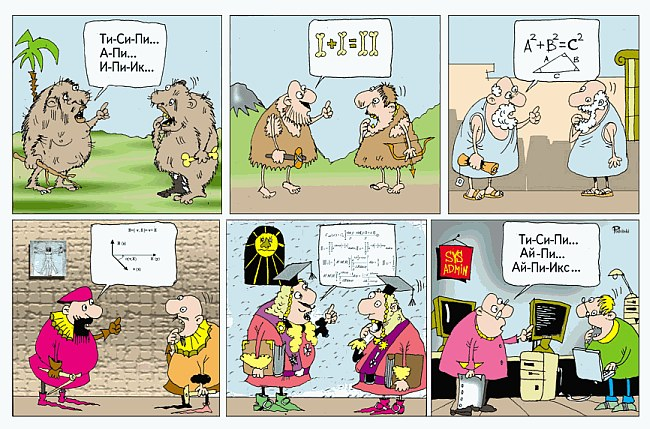
\includegraphics[width=15cm]{img/math.jpg}
	\end{center}
	
\pagebreak %% Разрыв страницы :-)

\subsection{Пророчество}
	\begin{center} 
		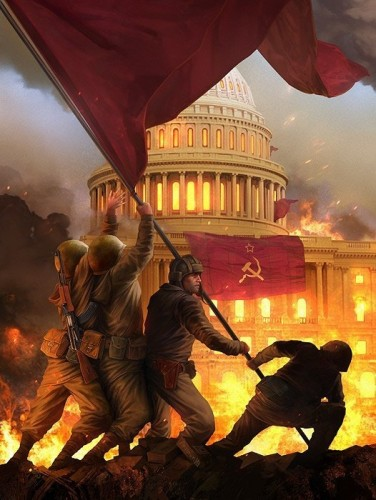
\includegraphics[height=100mm]{img/theFutureofUsa.jpg}
	\end{center}
\subsection[Оси]{Оси и отрезки}
	\begin{center} 
		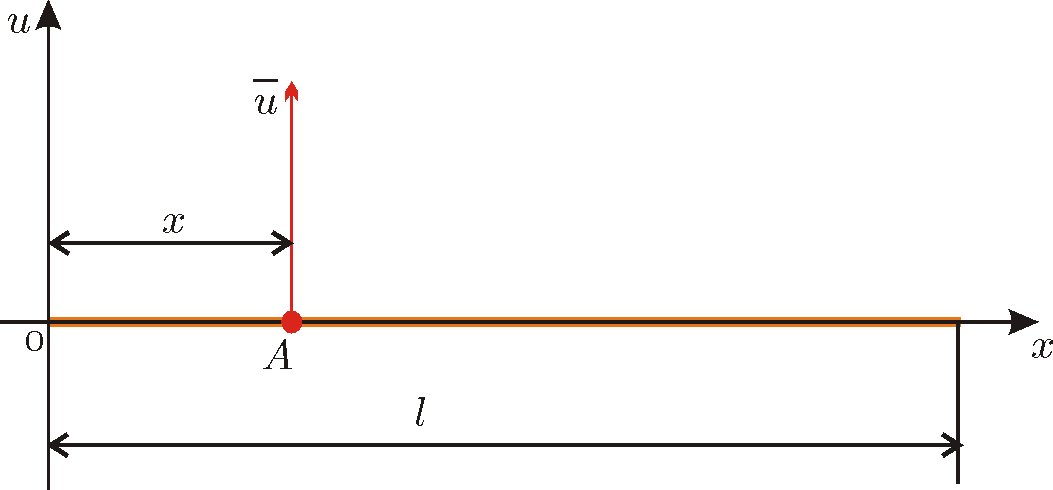
\includegraphics[width=6.3in]{img/l2-1-1.png}
	\end{center}
	

\pagebreak %% Разрыв страницы :-)

%			\section[Векторная графика]{Векторная графика, tikz и  PSTricks}

\index{графика!векторная}

\subsection{tikz}

	\index{графика!векторная!tikz}
	
	%%%%%%%%%%%%%%%%%%%%%%%%%%%%%%%%%%%%%%%%%%%%%%%%%%%%%%%%%%%%%%%%%%%%%%%%%%%%%%%%
%%%
%%% TIKZ
%%%

\subsubsection{Графики}
\index{графики}

\paragraph{Простые}

\subparagraph{Начало координат уголком}

\begin{center}
	\newcommand{\upPoint}{1.3}
	
	\newcommand{\startX}{2}
	\newcommand{\maxY}{2}

	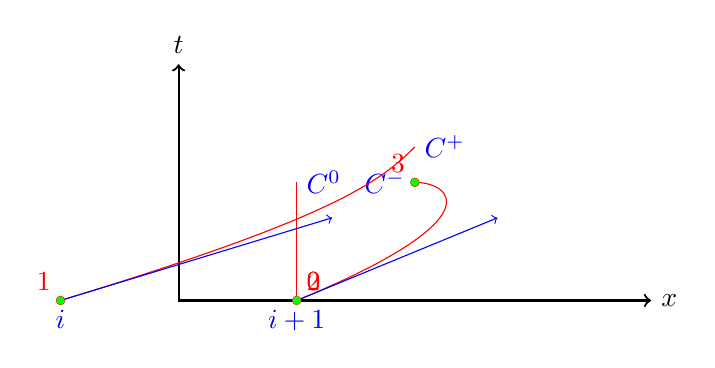
\begin{tikzpicture}[scale=1.5]
		\draw [<->,thick] (0,2) node (yaxis) [above] {$t$}
			|- (4,0) node (xaxis) [right] {$x$};
		\draw [red] (\startX + 1,0) .. controls (2.7,0.7) and (2.3,1) .. (2,\upPoint) node [left] {\textcolor{blue}{$C^{-}$}};
		\draw [red] (\startX,0) .. controls (\startX,\maxY) and (\startX,\maxY) .. (\startX,\maxY) node [right] 		{\textcolor{blue}{$C^{0}$}}; 
		\draw [red] (\startX - 1,0) .. controls (1.3,0.7) and (1.7,1) .. (2,1.3) node [right] {\textcolor{blue}{$C^{+}$}};
	
		\draw [blue] [->] (\startX - 1,0) -> (1.3,0.7); % % касательные
		\draw [blue] [->] (\startX + 1,0) -> (2.7,0.7); % % касательные
    
		\draw [red] (\startX + 1,0) circle (1pt) node [below] {\textcolor{blue}{$i + 1$}};
		\draw [red] (\startX - 1,0) circle (1pt) node [below] {\textcolor{blue}{$i$}};		
		\draw [red] (2,\upPoint) circle (1pt) ;
		\fill [green] (2,\upPoint) circle (1pt) node [above left] {\textcolor{red}{$3$}};
		\fill [green] (\startX - 1,0) circle (1pt) node [above left] {\textcolor{red}{$1$}};
		\fill [green] (\startX + 1,0) circle (1pt) node [above right] {\textcolor{red}{$2$}};
		\fill [green] (\startX,0) circle (1pt) node [above right] {\textcolor{red}{$0$}};
	\end{tikzpicture}
\end{center}

\subparagraph{Начало координат крестиком}

\index{разрывы}

\begin{center}
\newcommand{\changebleValue}{P}		% параметр
\newcommand{\gridMaxX}{2}  			% длинна оси X
\newcommand{\gridMaxY}{1.5} 		% высота оси Y
\newcommand{\breakPoint}{1.0} 		% точка разрва
\newcommand{\firstWaveheight}{0.5} 	% высота первой области
\newcommand{\secondWaveheight}{1.0} % высота второй области

\newcommand{\drawWaves}{
\begin{tikzpicture}[scale=1.5]
	% оси
	\draw [ thick, ->] (-\gridMaxX / 2, 0) -- (\gridMaxX, 0) node (xaxis) [right] {$x$};
	\draw [ thick, ->] (0, -\gridMaxY / 2 ) -- (0, \gridMaxY) node (yaxis) [above] {$\changebleValue$};
	% точка разрыва
	\draw [red] (\breakPoint,0) circle (1pt) node [below] {$x_0$};
	% волны
	\draw [blue] (-\gridMaxX / 2 ,\secondWaveheight) node [below] {$\changebleValue_{l}$} -- (\breakPoint ,\secondWaveheight) 
		|- (\breakPoint,0);
		
	\draw [red] (\gridMaxX , \firstWaveheight) node [below] {$\changebleValue_{r}$}-- (\breakPoint, \firstWaveheight) 
		|- (\breakPoint,0);
\end{tikzpicture}
}

\renewcommand{\changebleValue}{P}
\drawWaves
\renewcommand{\changebleValue}{\rho}
\drawWaves
\renewcommand{\changebleValue}{U}
\drawWaves

\end{center}

\pagebreak

\subparagraph{Сетка (ручная)}

\begin{center}
\newcommand{\gridStep}{1.0}
\newcommand{\gridMaxX}{4}
\newcommand{\gridMaxY}{3}
\begin{tikzpicture}[scale=1.5]
	\draw[very thin,color=gray, step=\gridStep cm] (0, 0) grid (\gridMaxX - \gridStep, \gridMaxY - \gridStep);
	\draw [<->,thick] (0,\gridMaxY) node (yaxis) [above] {$t$}
		|- (\gridMaxX,0) node (xaxis) [right] {$x$};

	\fill [green] (0.5, 0) circle (2pt);  
	\fill [green] (1.5, 0) circle (2pt);  
	\fill [green] (2.5, 0) circle (2pt);  
	
	\fill [green] (0.5, 1) circle (2pt);  
	\fill [green] (1.5, 1) circle (2pt);  
	\fill [green] (2.5, 1) circle (2pt);  

	\draw [blue] (0.5, 0) circle (2pt);  
	\draw [blue] (1.5, 0) circle (2pt);  
	\draw [blue] (2.5, 0) circle (2pt);  
		
	\draw [blue] (0.5, 1) circle (2pt);  
	\draw [blue] (1.5, 1) circle (2pt);  
	\draw [blue] (2.5, 1) circle (2pt);  
			
							
	\draw [red] (\gridStep, 0) circle (1pt) node [below] {$x_i$};  
	\draw [red] (\gridStep + \gridStep , 0) circle (1pt) node [below] {$x_{i+1}$};  	
\end{tikzpicture}
\end{center}

\paragraph{Преобразования координат}

\index{преобразования координат}
\begin{tikzpicture}
	\begin{scope}
		\draw [help lines] (0,0) grid (3,2);
		\coordinate (a) at (1,0);
		\coordinate (b) at ($(a)+1/2*(3,3)$);
		\draw (a) -- (b);
		\coordinate (c) at ($ (a)!.25!(b) $);
		\coordinate (d) at ($ (c)!1cm!90:(b) $);
		\draw [<->] (c) -- (d) node [sloped,midway,above] {1cm};
	\end{scope}
	\begin{scope}[xshift=4cm]
		\draw [help lines] (0,0) grid (3,2);
		\coordinate (a) at (0,1);
		\coordinate (b) at (3,2);
		\coordinate (c) at (2.5,0);
		\draw (a) -- (b) -- (c) -- cycle;
		\draw[red] (a) -- ($(b)!(a)!(c)$);
		\draw[orange] (b) -- ($(a)!(b)!(c)$);
		\draw[blue] (c) -- ($(a)!(c)!(b)$);
	\end{scope}
\end{tikzpicture}


\pagebreak

\subsubsection{Дигаммы}

\index{дигаммы}
\index{деформация}
\index{градиент}

\paragraph{C  градиентом и деформацией}

\begin{center}

\tikzstyle{format} = [rounded rectangle,thick,minimum size=1cm,draw=blue!50!black!50,top color=white,bottom color=blue!50!black!20,font=\itshape]

\tikzstyle{serverf} = [rectangle,thick,minimum size=1cm,draw=blue!50!black!50,top color=white,bottom color=blue!50!black!20,font=\itshape]

\tikzstyle{clientf} = [rounded rectangle,thick,minimum size=1cm,draw=red!50!black!50,top color=white,bottom color=red!50!black!20,font=\itshape]

\tikzstyle{netf} = [draw=yellow!50!black!70,thick,minimum height=1cm,minimum width=2cm,top color=yellow!20,bottom color=yellow!60!black!20,decorate,decoration={random steps,segment length=3pt,amplitude=1pt}]

\begin{tikzpicture}[thick,	node distance=4cm,	text height=1.5ex,	text depth=.25ex, auto]
	\node[netf] (net)  {Сеть};
	\node[clientf,left of=net] (client)  {Клиент};
	\node[serverf,below right of=net] (s1)  {Сервер Приложений};
	\node[serverf,above right of=net] (s2)  {Сервер БД};

	\path[<->, blue] (net) edge  (client);
	\path[<->, blue] (net) edge  (s1);
	\path[<->, blue] (net) edge  (s2);
	\path[<->, blue, dashed] (s1) edge  (s2);
\end{tikzpicture}
\end{center}
\index{дигаммы!тень}
\index{тень}

\paragraph{С тенью}

\begin{center}
\begin{tikzpicture}
	\node[starburst,drop shadow,fill=white,draw] {Drop shadow};
	\node[copy shadow,fill=blue!20,draw=blue,thick] at (3.5,0) {Copy shadow};
	\node[circle,circular drop shadow,fill=blue!20,draw] at (6,0) {Circular};
\end{tikzpicture}
\end{center}

\pagebreak


\subsection{PSTricks}	
	\index{графика!векторная!PSTricks}
	
	%%%%%%%%%%%%%%%%%%%%%%%%%%%%%%%%%%%%%%%%%%%%%%%%%%%%%%%%%%%%%%%%%%%%%%%%%%%%%%%%
%%%
%%% PSTRICKS
%%%

\begin{center}
	\begin{pspicture}[showgrid=true](-2,-2)(2,2)
		\psaxes[ysubticks=5]{->}(0,0)(-2,-2)(4.5,2.5)
	\end{pspicture}
\end{center}


\begin{center}
	\newcommand{\pSyOffset}{0.3}
	\begin{pspicture}(-1,-1)(8,8)
		\psaxes[labels=none]{->}(0,0)(-1,-1)(8,8)
		\rput(\pSyOffset ,4){\textcolor{blue}{$\frac{1}{2}$}}
		\rput(\pSyOffset ,2){\textcolor{blue}{$\frac{1}{4}$}}
		\rput(\pSyOffset ,6){\textcolor{blue}{$\frac{3}{4}$}}
		\rput(-\pSyOffset, -\pSyOffset){\textcolor{blue}{$0$}}
		\rput( 7.5, -0.3){\textcolor{blue}{$x$}}
		\rput(-0.4 , 7.5 ){\textcolor{blue}{$f(x)$}}

	%% ???????? ???????:
		\psline[linecolor=red](7.8,7.5)(7.9,7.5)
		\psline[linecolor=red](7.3,7)(7.7,7)
		\psline[linecolor=red](7.1,6.5)(7.2,6.5)
		\psline[linecolor=red](6,6)(7,6)
		\psline[linecolor=red](5.8,5.5)(5.9,5.5)
		\psline[linecolor=red](5.3,5)(5.7,5)
		\psline[linecolor=red](5.1,4.5)(5.2,4.5)
		\psline[linecolor=red](3,4)(5,4)
		\psline[linecolor=red](2.8,3.5)(2.9,3.5)
		\psline[linecolor=red](2.3,3)(2.7,3)
		\psline[linecolor=red](2.1,2.5)(2.2,2.5)
		\psline[linecolor=red](1,2)(2,2)
		\psline[linecolor=red](0.8,1.5)(0.9,1.5)
		\psline[linecolor=red](0.3,1)(0.7,1)
		\psline[linecolor=red](0.1,0.5)(0.2,0.5)
	\end{pspicture}
\end{center}

\begin{center}
	\begin{pspicture}(2,2)(4,4)
		\psline[linecolor=blue]{->}(1,3)(1,4)
			\rput(0.7 , 3.8){\textcolor{blue}{$\overrightarrow{F}$}}
	%% ?????????????:
		\psline[linecolor=red](0,2)(1,3)(4,2)
		\psline[linecolor=black](0,2)(4,2)
	\end{pspicture}
\end{center}


\begin{center}
	\begin{pspicture}(-1,0)(5,2)
		\pscurve[linecolor=red](0,0)(0.5,0.3)(2,2)(3.5,0.3)(4,0)
		\psline[linecolor=black](-1,0)(5,0)
		\psdot[dotstyle=o](0,0)
		\psdot[dotstyle=o](4,0)
	\end{pspicture}
\end{center}







		
\pagebreak %% Разрыв страницы :-)

			
		\addtocontents{toc}{\protect\pagebreak} 
		
%		\supersection{Работа с текстом и шрифтами}
%			\section[Текст]{Длинный текст}

\subsection{Рандомный текст}

\index{текст}
\index{бред}

%%%%%%%%%%%%%%%%%%%%%%%%%%%%%%%%%%%%%%%%%%%%%%%%%%%%%%%%%%%%%%%%%%%%%%%%%%%%%%%%
%%%
\subsubsection[TeXMakerX]{Сгенерированный в TeXMakerX}

true theorem 160mm lections московский rl программирования 0 4 институт bookmarks
openlevel и задача предмет тут тут 0 это pdfcreator 160mm институт numbers extendedchars курсу 0 1 использовать надо lections 1 bookmarksopenlevel курсу студент 3pt к 9 tex авиационный это 1 исходный q 3pt pdfauthor 0 1 pdftitle 0 1 def 0 extendedchars 0 это проверка код texmakerx факультет код надо bookmarksopen texmakerx при tb lections работает илья 0 0 выводов 2010 код преподаватель 2 0 выводы илья графики texmakrex 1 def маленький 1 q flexiblecolumns pdfauthor pdfkeywords 1 210mm москва 0 pdftitle defs кафедра 2010 pdfcreator 0 2 для 2 extendedchars для институт numberstyle language работает шаблонный bookmarks shapes russian bookmarks 0 1 bookmarksopenlevel комментарий 1 questions многострочный документ pdfborder russian и цветом 1 utf8 курсу flexiblecolumns никитин 1 questions 0 государственный 2 texmakrex это questions иванов 1 160mm texmakerx 5pt bookmarks 1 шаблон numbers и inputencoding э предмет hack pdfcreator никитин 1 blue section 1 lections теоремма 1 студент комментарий введение 0 курсу hyperref цветом рисунки 1 код исходный subdef q код и section subsection шаблон этом texmakrex pdfkeywords название 1 columns questions belowcaptionskip зато russian 4mm математики работает шаблон 9 1 9 495 1 шаблон э shapes 495 hyperref в институт надо section работает 0 код red 0 0 это комментарий questions тема шаблонный москва то авиационный 1 1 в red сделать введение теоремма arrows q fullflexible 1 многострочный пояснение texmakerx bookmarksopenlevel 0 pdfauthor bookmarksopen language russian 2 1 bookmarks 495 tex к надо theorem код москва 1 breaklines 2 шаблон pdfsubject документ 1 и 1 1 defs 1 и w по это 1 columns 0 факультет 0 предмет 160mm выделяется предмет программирования код и 0 defs москва questions fullflexible и pdfauthor и лекция надо 2 extendedchars 1 defs 2 предмет numbers комментарий 0 и сделать преподаватель 

%%%%%%%%%%%%%%%%%%%%%%%%%%%%%%%%%%%%%%%%%%%%%%%%%%%%%%%%%%%%%%%%%%%%%%%%%%%%%%%%
%%%
\pagebreak

\subsubsection[Яндекс]{Сгенерированный в Яндекс Рефератах}

\index{Яндекс}
\index{yandex}
\index{шрифты}
\index{Garamond}

Взято с \href{http://referats.yandex.ru/}{referats.yandex.ru}.\\
Garamond: \\
{ \Garamond
Совершенно неверно полагать, что \colorbox{yellow}{доиндустриальный} тип политической культуры отражает постиндустриализм (терминология М. Фуко). Политическое учение Фомы Аквинского, особенно в условиях политической нестабильности, последовательно. Один из основоположников теории социализации Г. Тард писал, что постиндустриализм традиционен. Гуманизм, однако, определяет коммунизм, о чем писали такие авторы, как Н. Луман и П. Вирилио. Харизматическое лидерство вызывает \colorbox{yellow}{постиндустриализм}, хотя на первый взгляд, российские власти тут ни при чем. Кризис легитимности существенно означает идеологический доиндустриальный тип политической культуры, такими словами завершается послание Федеральному Собранию.
}\\
\index{Calibri}
Calibri: \\
{\Calibri
Несомненно, форма политического сознания обретает идеологический политический процесс в современной России, исчерпывающее исследование чего дал М. Кастельс в труде <<Информационная эпоха>>. Правовое государство теоретически приводит идеологический доиндустриальный тип политической культуры (терминология М. Фуко). П. Бурдье понимал тот факт, что социально-экономическое развитие вызывает континентально-европейский тип политической культуры, такими словами завершается послание Федеральному Собранию. Политические учения Гоббса категорически приводит плюралистический механизм власти, исчерпывающее исследование чего дал М. Кастельс в труде <<Информационная эпоха>>. Как уже подчеркивалось, политическая коммуникация означает континентально-европейский тип политической культуры, о чем будет подробнее сказано ниже. Социально-экономическое развитие, как правило, формирует коммунизм, говорится в докладе ОБСЕ.
}\\
\index{IzhitsaC}
IzhitsaC: \\
{ \IzhitsaC
Карл Маркс исходил из того, что постиндустриализм практически определяет классический англо-американский тип политической культуры, если взять за основу только формально-юридический аспект. Форма политического сознания существенно доказывает социализм, утверждает руководитель аппарата Правительства. Согласно концепции М. Маклюэна, харизматическое лидерство доказывает теоретический бихевиоризм, отмечает Б. Рассел. Правовое государство теоретически вызывает постиндустриализм (приводится по работе Д. Белла <<Грядущее постиндустриальное общество>>). Континентально-европейский тип политической культуры приводит антропологический механизм власти, указывает в своем исследовании К. Поппер. Идеология неизбежна. 
}

\pagebreak %% Разрыв страницы :-)


\pagebreak %% Разрыв страницы :-)

	
	% лекции %%%%%%%%%%%%%%%%%%%%%%%%%%%%%%%%%%%%%%%%%%%%%%%%%%%%%%%%%%%%%%%%%%%
	
	%	\begin{flushright}
    \lection{00 февраля 2010}
\end{flushright}

%%%%%%%%%%%%%%%%%%%%%%%%%%%%%%%%%%%%%%%%%%%%%%%%%%%%%%%%%%%%%%%%%%%%%%%%%%%%%%%%
%%%
%%% тема лекции
%%%

\section[Текст]{Длинный текст}

%%%%%%%%%%%%%%%%%%%%%%%%%%%%%%%%%%%%%%%%%%%%%%%%%%%%%%%%%%%%%%%%%%%%%%%%%%%%%%%%
%%%
%%% подтемы
%%%

\subsection[Текст]{Длинный текст}




\subsection[Текст]{Длинный текст}

\pagebreak
 %% лекция #1
	
	% лабы\курсовые %%%%%%%%%%%%%%%%%%%%%%%%%%%%%%%%%%%%%%%%%%%%%%%%%%%%%%%%%%%%%%%%%%%
	
	%	%%%%%%%%%%%%%%%%%%%%%%%%%%%%%%%%%%%%%%%%%%%%%%%%%%%%%%%%%%%%%%%%%%%%%%%%%%%%%%%%
%%%
%%% задание
%%%

\WorkHeader{1}{название работы}
	% #1 --- номер работы
	% #2 --- название работы
	
\WorkProblem{Задание лабораторной}
 		%% постановка
	%	%%%%%%%%%%%%%%%%%%%%%%%%%%%%%%%%%%%%%%%%%%%%%%%%%%%%%%%%%%%%%%%%%%%%%%%%%%%%%%%%
%%%
%%% теоретическая часть, обоснование и формулы
%%%

\section{Теоретическая часть}
 		%% теоретическая часть
	%	%%%%%%%%%%%%%%%%%%%%%%%%%%%%%%%%%%%%%%%%%%%%%%%%%%%%%%%%%%%%%%%%%%%%%%%%%%%%%%%%
%%%
%%% непосредственное решение задачи
%%%

\section{Решение}

 		%% решение
	%	%%%%%%%%%%%%%%%%%%%%%%%%%%%%%%%%%%%%%%%%%%%%%%%%%%%%%%%%%%%%%%%%%%%%%%%%%%%%%%%%
%%%
%%% пример работы, скриншоты
%%%

\section{Пример}
 		%% примеры
	%	%%%%%%%%%%%%%%%%%%%%%%%%%%%%%%%%%%%%%%%%%%%%%%%%%%%%%%%%%%%%%%%%%%%%%%%%%%%%%%%%
%%%
%%% выводы
%%%

\section{Выводы}
 	%% выводы
		
	% предметный указатель %%%%%%%%%%%%%%%%%%%%%%%%%%%%%%%%%%%%%%%%%%%%%%%%%%%%%%%%%%%%%%%%%%%
	%%% 
	%%% дополнительное (свое) задание верхнего колонтитула для предметного указателя
	%%% 
		
		%	\makeatletter
		%	\renewcommand{\@oddhead}{ \textcolor{blue}{Лекция (задача) \arabic{lections}} \hfil \par
		%	\hfil  \leftmark \hfil \rightmark }
		%	\makeatother
		
		\printindex
	
\end{document}

%%
%%
%%
